
\documentclass[border=8pt, multi, tikz]{standalone}
\usepackage{amsmath}
\usepackage{amssymb}
\usepackage{import}
\subimport{figures/architecture/}{init}
\usetikzlibrary{positioning}
\usetikzlibrary{calc}
\usetikzlibrary{fit}
\usetikzlibrary{3d}
\usetikzlibrary{decorations.pathreplacing}

% --- arch_overview color palette ---
\colorlet{EncColor}{blue!18}
\colorlet{EncBandColor}{blue!50}
\colorlet{SlotColor}{yellow!75}
\colorlet{NCAColor}{green!35}
\colorlet{NCABandColor}{green!70}
\colorlet{EmbedColor}{green!12}
\colorlet{ReadoutColor}{red!18}

\newcommand{\copymidarrow}{\tikz \draw[-Stealth,line width=0.8mm,draw={rgb:blue,4;red,1;green,1;black,3}] (-0.3,0) -- ++(0.3,0);}

\begin{document}
\begin{tikzpicture}
\tikzstyle{connection}=[ultra thick,every node/.style={sloped,allow upside down},draw=\edgecolor,opacity=0.7]
\tikzstyle{flowarrow}=[-Stealth, line width=0.5mm, opacity=0.85]
\tikzstyle{condarrow}=[-Stealth, line width=0.5mm, dashed,
    draw={rgb:blue,5;magenta,2;black,2}, opacity=0.9]
\tikzstyle{tflayer}=[draw, rounded corners=1.2pt, line width=0.3pt,
    minimum width=0.4cm, minimum height=2.4cm, inner sep=1pt]

% =============================================================
% LEFT: spec -> encoder -> latent (non-spatial)
% =============================================================

% --- input game spec ---
\node[draw, rounded corners=2pt, fill={gray!8},
      font=\footnotesize\ttfamily, align=left, inner sep=4pt,
      text width=3.6cm, anchor=east] (spec) at (-8.5,0)
{objects\\
=========\\
\textbf{Player} \textbf{Crate}\\
\textbf{Wall} \textbf{Target}\\
=========\\
rules\\
=========\\
{[}\textbf{>} Player | Crate{]}\\
~->{[}|\textbf{>}P. \textbf{>}Cr.{]}\\
=========\\
winconditions\\
=========\\
all Crate on Target};
\node[font=\small\itshape, anchor=south] at (spec.north) {game spec};

% --- Encoder block: 2 self-attn + 1 cross-attn ---
\node[tflayer, fill=EncColor]   (encS1) at (-6.8, 0) {};
\node[tflayer, fill=EncColor, right=0.08cm of encS1] (encS2) {};
\node[tflayer, fill=EncBandColor, right=0.08cm of encS2] (encX)  {};
\node[font=\scriptsize, rotate=90, inner sep=0pt] at (encS1) {self-attn};
\node[font=\scriptsize, rotate=90, inner sep=0pt] at (encS2) {self-attn};
\node[font=\scriptsize, rotate=90, inner sep=0pt, text=white!92!black]
    at (encX) {$K$-query x-attn};
\node[draw, rounded corners=2pt, line width=0.45pt, fit=(encS1)(encX),
      inner sep=3pt] (enc) {};
\node[font=\small\bfseries, anchor=south] at (enc.north)
    {Encoder $\mathrm{Enc}_\phi$};

% --- Latent (slot/FiLM/VQ-agnostic) ---
\node[draw, rounded corners=1.5pt, fill=SlotColor, line width=0.4pt,
      minimum width=0.55cm, minimum height=2.6cm, anchor=center]
      (slots) at (-4.4, 0) {};
\node[font=\small\bfseries, anchor=south] at (slots.north) {latent $z$};

% --- spec -> enc -> latent ---
\draw[flowarrow] (spec.east) -- (enc.west);
\draw[flowarrow] (enc.east)  -- (slots.west);

% =============================================================
% RIGHT: dynamics row (s_t/embed -> NCA body -> readout/s_{t+1})
% Box height=20, depth=20, scale=0.2 => visible y-z face is 4cm x 4cm,
% sized to the 3.6cm sokoban level images.
% =============================================================

% --- s_t (embed box, image projected on the east/front face) ---
\pic[shift={(-2.2,0,0)}] at (0,0,0)
    {Box={
        name=embed,
        caption= ,
        xlabel={{,}},
        zlabel={},
        fill=EmbedColor,
        height=20,
        width=2.5,
        depth=20
        }
    };
\node[canvas is zy plane at x=-1.7] (sin) at (0,0)
    {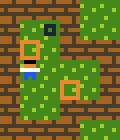
\includegraphics[width=3.6cm,height=3.6cm]{figures/architecture/state_in.png}};
\path let \p1=(embed-south) in
    node[font=\large, anchor=north] at (\x1, -2.5cm) {$s_t$};

% --- NCA body: a single RightBandedBox with n_layers bands;
%     the whole body is iterated n_repeats times (loop arrow below).
\pic[shift={(0.4,0,0)}] at (0,0,0)
    {RightBandedBox={
        name=nca,
        caption= ,
        xlabel={{,,}},
        zlabel={},
        fill=NCAColor,
        bandfill=NCABandColor,
        height=20,
        width={1.6,1.6,1.6},
        depth=20
        }
    };
\path let \p1=(nca-south) in
    node[font=\small, anchor=north] at (\x1, -2.7cm) {$3{\times}3$ conv (per layer)};

% Brace + label for n_layers (just above body). Mirrored so the apex
% points UP at the label.
\path let \p1 = (nca-west), \p2 = (nca-east) in
    coordinate (braceLeft)  at (\x1-0.05cm, 2.20cm)
    coordinate (braceRight) at (\x2+0.05cm, 2.20cm);
\draw[decorate, decoration={brace, amplitude=6pt, raise=4pt, mirror}, line width=0.4pt]
    (braceRight) -- (braceLeft);
\node[font=\small\itshape, anchor=south]
    at ($(braceLeft)!0.5!(braceRight)+(0,0.45cm)$) {$n_\text{layers}$};

% --- s_{t+1} (readout box, image projected on east/front face) ---
\pic[shift={(5.6,0,0)}] at (0,0,0)
    {Box={
        name=readout,
        caption= ,
        xlabel={{,}},
        zlabel={},
        fill=ReadoutColor,
        height=20,
        width=2.5,
        depth=20
        }
    };
\node[canvas is zy plane at x=6.1] (sout) at (0,0)
    {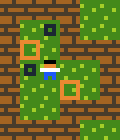
\includegraphics[width=3.6cm,height=3.6cm]{figures/architecture/state_out.png}};
\path let \p1=(readout-south) in
    node[font=\large, anchor=north] at (\x1, -2.5cm) {$s_{t+1}$};

% --- forward connections through dynamics row ---
\draw[connection] (embed-east) -- node {\midarrow} (nca-west);
\draw[connection] (nca-east)   -- node {\midarrow} (readout-west);

% --- Loop arrow below the body (n_repeats), routed below caption text.
\path let \p1 = (nca-east), \p2 = (nca-west) in
    coordinate (loopOutR)  at (\x1+0.4cm, \y1)
    coordinate (loopOutRD) at (\x1+0.4cm, -4.0cm)
    coordinate (loopInLD)  at (\x2-0.4cm, -4.0cm)
    coordinate (loopInL)   at (\x2-0.4cm, \y2);
\draw[-Stealth, line width=0.7mm, opacity=0.32, rounded corners=10pt]
    (nca-east) -- (loopOutR) -- (loopOutRD) -- (loopInLD) -- (loopInL) -- (nca-west);
\node[font=\small\itshape, opacity=0.7]
    at ($(loopOutRD)!0.5!(loopInLD)+(0,-0.40)$) {$\times\, n_\text{repeats}$};

% =============================================================
% Cross-attention: latent -> NCA body, routed above the figure.
% Apply at every layer (every step inside the loop).
% =============================================================
\path let \p1 = (slots.north), \p2 = (nca-north) in
    coordinate (slotsTop)   at (\x1, \y1)
    coordinate (overslots)  at (\x1, 4.5cm)
    coordinate (overnca)    at (\x2, 4.5cm)
    coordinate (ncaTopIn)   at (\x2, \y2+0.10cm);

\draw[condarrow, rounded corners=8pt, line width=0.5mm]
    (slotsTop) -- (overslots) -- (overnca) -- (ncaTopIn);

\node[font=\footnotesize, text=blue!55!black, anchor=south, align=center]
    at ($(overslots)!0.5!(overnca)+(0,0.10cm)$)
    {keys, values \textit{(every layer)}};

\end{tikzpicture}
\end{document}
